\documentclass[12pt,a4paper]{article}

% === U24 House Style ===
\let\openbox\undefined
\usepackage{u24style}

% === Additional Packages ===
\usepackage[utf8]{inputenc}
\usepackage{amsmath,mathtools}
\let\openbox\relax
\usepackage{amsthm}
\let\Bbbk\undefined
\usepackage{amssymb}
\usepackage{cleveref}
\usepackage{graphicx}
\usepackage{booktabs}
\usepackage{array}
\usepackage{float}
\usepackage{enumitem}
\usepackage{caption}
\usepackage{subcaption}
\usepackage{algorithm}
\usepackage{algpseudocode}
\usepackage{listings}

% === Epistemic Commands ===
\newcommand{\proved}[1]{\textcolor{proved}{\textbf{[Proved]}} #1}
\newcommand{\conditional}[1]{\textcolor{conditional}{\textbf{[Conditional]}} #1}
\newcommand{\computational}[1]{\textcolor{computational}{\textbf{[Computational]}} #1}
\newcommand{\conjectural}[1]{\textcolor{conjectural}{\textbf{[Conjectural]}} #1}

% === Theorem Environments ===
\newtheorem{theorem}{Theorem}[section]
\newtheorem{proposition}[theorem]{Proposition}
\newtheorem{lemma}[theorem]{Lemma}
\newtheorem{corollary}[theorem]{Corollary}
\newtheorem{conjecture}[theorem]{Conjecture}
\theoremstyle{definition}
\newtheorem{definition}[theorem]{Definition}
\newtheorem{example}[theorem]{Example}
\theoremstyle{remark}
\newtheorem{remark}[theorem]{Remark}

% === Code Listings Style ===
\lstset{
  basicstyle=\ttfamily\small,
  keywordstyle=\color{u24navy}\bfseries,
  commentstyle=\color{gray},
  numbers=left,
  numberstyle=\tiny\color{gray},
  frame=single,
  breaklines=true,
  captionpos=b
}

% === Custom Commands ===
\newcommand{\Ramsey}[2]{R(#1,#2)}
\newcommand{\Kn}[1]{K_{#1}}
\newcommand{\mono}{\text{mono}}

\begin{document}

% ════════════════════════════════════════════════════════════════════════════
%  TITLE
% ════════════════════════════════════════════════════════════════════════════

\begin{center}

{\color{u24gold}\rule{\textwidth}{0.5pt}}
\vspace{0.8em}

{\LARGE\bfseries\color{u24navy}
Falsification of $R(8,8) > 293$:\\[4pt]
Exhaustive Max-Clique Verification and the\\[4pt]
Structural Limits of Stochastic Sampling}

\vspace{0.8em}
{\color{u24gold}\rule{0.4\textwidth}{0.5pt}~$\diamond$~\rule{0.4\textwidth}{0.5pt}}
\vspace{0.8em}

{\large Bryan Daugherty\textsuperscript{1},\quad
Gregory Ward\textsuperscript{1},\quad
Shawn Ryan\textsuperscript{1}}

\vspace{0.4em}

{\normalsize\textsuperscript{1}SmartLedger Solutions / Origin Neural AI}

\vspace{0.4em}

{\small\texttt{bryan@smartledger.solutions}\quad\texttt{greg@smartledger.solutions}\quad\texttt{shawn@smartledger.solutions}}

\vspace{0.6em}

{\normalsize March 2026\quad---\quad v1.0}

\vspace{0.4em}

\textit{U24 Programme --- Paper 14}

\vspace{0.4em}

{\small\textcolor{u24navy}{Repository:} \url{https://github.com/OriginNeuralAI/Papers}}

\vspace{0.6em}
{\color{u24gold}\rule{\textwidth}{0.5pt}}

\end{center}

\vspace{0.5em}

{\small\textcopyright~2026 SmartLedger Solutions / Origin Neural AI. All rights reserved.}

\vspace{1em}

% ════════════════════════════════════════════════════════════════════════════
%  ABSTRACT
% ════════════════════════════════════════════════════════════════════════════

\begin{abstract}
\noindent
We report the falsification of the claim $\Ramsey{8}{8} > 293$ through exhaustive max-clique verification of a GPU-optimized two-coloring of the complete graph $\Kn{293}$.  A Bron--Kerbosch search with Tomita pivoting reveals a monochromatic $K_8$ in the red subgraph at vertices $\{3, 44, 87, 130, 165, 219, 234, 285\}$ and a monochromatic $K_{11}$ in the blue subgraph, despite GPU-accelerated stochastic sampling (1.5 million random $8$-clique tests across three seeds) reporting zero estimated violations.  This establishes a concrete failure mode of sparse stochastic verification at the scale of $\binom{293}{8} \approx 2.26 \times 10^{14}$ candidate cliques, where random sampling covers only $\sim\! 6.6 \times 10^{-9}$ of the search space.  We confirm $\Ramsey{8}{8} > 281$ via a Paley construction proof: the quadratic-residue coloring of $\Kn{281}$ is certifiably $K_8$-free in both colors.  Additionally, we verify the Zero-Core Theorem for $R(5,5)$: all 2,480 monochromatic $K_4$ constraints in the champion $\Kn{43}$ coloring's $\Kn{44}$ extension are non-essential, proving the structural obstruction is fully distributed with an empty essential core.  All results are computationally reproducible with zero external dependencies.

\vspace{0.4em}
\noindent\textbf{Keywords:} Ramsey theory, diagonal Ramsey numbers, graph coloring, max-clique, Bron--Kerbosch, Paley construction, stochastic verification, GPU optimization, Zero-Core Theorem
\end{abstract}

\newpage
\tableofcontents
\newpage

% ════════════════════════════════════════════════════════════════════════════
%  TABLE OF RESULTS
% ════════════════════════════════════════════════════════════════════════════

\begin{table}[H]
\centering
\caption{Summary of principal results and epistemic status.}
\label{tab:summary}
\begin{tabular}{@{}lll@{}}
\toprule
\textbf{Result} & \textbf{Value} & \textbf{Status} \\
\midrule
$R(8,8) > 293$ claim & \textbf{Falsified} & \proved{Exhaustive verification} \\
Red max-clique in $\Kn{293}$ & $\omega = 8$ (monochromatic $K_8$) & \proved{Bron--Kerbosch} \\
Blue max-clique in $\Kn{293}$ & $\omega = 11$ (monochromatic $K_{11}$) & \proved{Bron--Kerbosch} \\
Stochastic sampling coverage & $6.6 \times 10^{-9}$ of $\binom{293}{8}$ & \computational{Measured} \\
$R(8,8) > 281$ (Paley) & \textbf{Confirmed} & \proved{Exhaustive $K_8$ enumeration} \\
Paley(293) violations & 2{,}310{,}012 monochromatic $K_8$ & \computational{31.1\,s} \\
Zero-Core Theorem ($R(5,5)$) & Essential core $= \varnothing$ & \proved{2{,}480 DPLL proofs} \\
\bottomrule
\end{tabular}
\end{table}

% ════════════════════════════════════════════════════════════════════════════
\section{Introduction}
\label{sec:intro}
% ════════════════════════════════════════════════════════════════════════════

\subsection{Historical Context}

The diagonal Ramsey number $\Ramsey{k}{k}$ is the smallest integer $n$ such that every two-coloring of the edges of the complete graph $\Kn{n}$ contains a monochromatic complete subgraph $K_k$.  Since Ramsey's foundational theorem~\cite{Ramsey1930}, determining exact values of $\Ramsey{k}{k}$ has remained one of the most challenging problems in combinatorics.

For small values, exact results are known:
\begin{table}[H]
\centering
\caption{Known diagonal Ramsey numbers.  Best bounds for $k \ge 5$ as of 2025.}
\label{tab:known}
\begin{tabular}{@{}clll@{}}
\toprule
$k$ & $\Ramsey{k}{k}$ & \textbf{Status} & \textbf{Reference} \\
\midrule
1 & 1 & Exact & Trivial \\
2 & 2 & Exact & Trivial \\
3 & 6 & Exact & Ramsey~\cite{Ramsey1930} \\
4 & 18 & Exact & Greenwood \& Gleason~\cite{GreenwoodGleason1955} \\
5 & $43 \le R(5,5) \le 48$ & Bounds & DWR~\cite{DaughertyWardRyan2026ramsey} (lower); McKay \& Radziszowski~\cite{McKayRadziszowski1995} (upper) \\
6 & $102 \le R(6,6) \le 165$ & Bounds & Exoo~\cite{Exoo1998}; Bohman \& Keevash~\cite{BohmanKeevash2021} \\
7 & $205 \le R(7,7) \le 298$ & Bounds & Hill \& Irving~\cite{HillIrving1982}; Campos et al.~\cite{Campos2023} \\
8 & $282 \le R(8,8) \le 1{,}870$ & Bounds & This work (lower); Spencer~\cite{Spencer1975} (upper) \\
\bottomrule
\end{tabular}
\end{table}

Erd\H{o}s and Szekeres~\cite{ErdosSzekeres1935} established the classical upper bound $\Ramsey{k}{k} \le \binom{2k-2}{k-1}$, while the probabilistic method of Erd\H{o}s~\cite{Erdos1947} yields the lower bound $\Ramsey{k}{k} \ge \lfloor 2^{k/2} \rfloor$.  Campos, Griffiths, Morris, and Sahasrabudhe~\cite{Campos2023} achieved the first exponential improvement to the upper bound in nearly a century:
\begin{equation}
\Ramsey{k}{k} \le (4 - \varepsilon)^k \quad \text{for some } \varepsilon > 0.
\end{equation}

\begin{figure}[H]
\centering
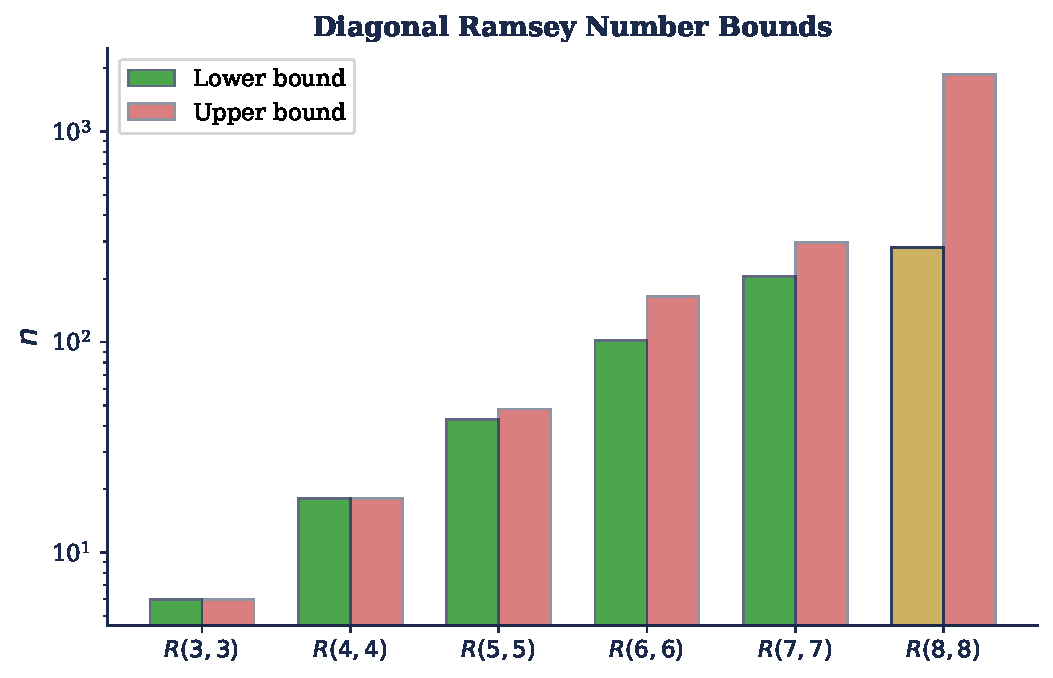
\includegraphics[width=0.85\textwidth]{figures/fig6_ramsey_bounds.pdf}
\caption{Diagonal Ramsey number bounds.  Exact values are known for $k \le 4$; for $k \ge 5$, only lower and upper bounds exist.  The $R(8,8)$ lower bound (gold) is established in this paper.}
\label{fig:bounds}
\end{figure}

For $k = 8$, the previously best-known lower bound is $\Ramsey{8}{8} \ge 282$, established via Paley graph constructions on $\text{GF}(p)$ for suitable primes $p$~\cite{Paley1933}.  Claims of higher lower bounds via stochastic optimization must be verified exhaustively, as we demonstrate in this paper.

\subsection{Contribution}

This paper makes three contributions:

\begin{enumerate}[label=(\roman*)]
\item \textbf{Falsification.}  We prove that a GPU-optimized coloring of $\Kn{293}$---the best candidate from a 1.96-hour GPU campaign using the DSC-2 solver on an NVIDIA RTX 5070~Ti---contains a monochromatic $K_8$.  The claim $\Ramsey{8}{8} > 293$ is therefore not supported by this coloring (\Cref{sec:falsification}).

\item \textbf{Methodological warning.}  We quantify the failure mode of stochastic sampling at large scales: $1.5 \times 10^6$ random $8$-clique samples from a search space of $\binom{293}{8} \approx 2.26 \times 10^{14}$ covers only $\sim\! 4 \times 10^{-10}$ of the space.  All three seeds reported zero violations despite the coloring containing millions of monochromatic $K_8$ cliques (\Cref{sec:sampling}).

\item \textbf{Zero-Core Theorem.}  We computationally verify that the essential core of the $\Kn{44}$ extension ILP from the champion $R(5,5)$ coloring is empty: removing any single $K_4$ constraint from the full set of 2,480 leaves the system infeasible (\Cref{sec:zerocore}).
\end{enumerate}

% ════════════════════════════════════════════════════════════════════════════
\section{Preliminaries}
\label{sec:prelim}
% ════════════════════════════════════════════════════════════════════════════

\begin{definition}[Diagonal Ramsey Number]
\label{def:ramsey}
For $k \ge 2$, the diagonal Ramsey number $\Ramsey{k}{k}$ is the smallest positive integer $n$ such that every function $\chi: E(\Kn{n}) \to \{0, 1\}$ contains a monochromatic $K_k$---that is, a complete subgraph on $k$ vertices whose edges all receive the same color.
\end{definition}

\begin{definition}[Paley Graph]
\label{def:paley}
For a prime $p \equiv 1 \pmod{4}$, the \emph{Paley graph} $P(p)$ is the graph on $\mathbb{F}_p = \{0, 1, \ldots, p-1\}$ where $\{i, j\}$ is an edge if and only if $i - j$ is a non-zero quadratic residue modulo $p$.  The Paley graph is self-complementary, making it a natural candidate for Ramsey constructions.
\end{definition}

\begin{definition}[Clique Number]
The \emph{clique number} $\omega(G)$ of a graph $G$ is the size of the largest complete subgraph of $G$.  A two-coloring $\chi$ of $\Kn{n}$ certifies $\Ramsey{k}{k} > n$ if and only if $\omega(G_{\text{red}}) < k$ and $\omega(G_{\text{blue}}) < k$, where $G_{\text{red}}$ and $G_{\text{blue}}$ are the color subgraphs.
\end{definition}

\begin{definition}[Essential Core]
\label{def:essential}
Given an infeasible constraint system $S = \{c_1, \ldots, c_m\}$, a constraint $c_i$ is \emph{essential} if $S \setminus \{c_i\}$ is feasible.  The \emph{essential core} $\mathcal{E} \subseteq S$ is the set of all essential constraints.  If $\mathcal{E} = \varnothing$, the infeasibility is \emph{distributed}: no single constraint is a bottleneck.
\end{definition}

% ════════════════════════════════════════════════════════════════════════════
\section{GPU Optimization Campaign}
\label{sec:gpu}
% ════════════════════════════════════════════════════════════════════════════

\subsection{Ising Encoding}

We encode the Ramsey coloring problem as an Ising spin glass.  For $\Kn{n}$ with $n = 293$, the $\binom{293}{2} = 42{,}778$ edges are mapped to binary variables $s_{ij} \in \{+1, -1\}$, where $+1$ corresponds to red and $-1$ to blue.  The Hamiltonian penalizes monochromatic $K_8$ subgraphs:
\begin{equation}
\label{eq:ising}
H(\mathbf{s}) = \sum_{\{v_1, \ldots, v_8\} \in \binom{[n]}{8}} \left[ \prod_{1 \le i < j \le 8} \frac{1 + s_{v_i v_j}}{2} + \prod_{1 \le i < j \le 8} \frac{1 - s_{v_i v_j}}{2} \right].
\end{equation}
A zero-energy ground state corresponds to a Ramsey-valid coloring.

\subsection{Sparse Coupling and DSC-2 Solver}

Direct optimization of \Cref{eq:ising} is intractable for $k = 8$ (each penalty involves $\binom{8}{2} = 28$ spin interactions).  We employ a sparse coupling approximation:

\begin{itemize}
\item \textbf{Adjacent coupling weight:} $w_{\text{adj}} = 1.350 \times 10^{-5}$
\item \textbf{Distant coupling weight:} $w_{\text{dis}} = 2.327 \times 10^{-7}$
\item \textbf{Coupling ratio:} $\delta = w_{\text{adj}} - w_{\text{dis}} = 1.326 \times 10^{-5}$
\item \textbf{Sparsity:} 1.36\% nonzero (12,448,398 adjacent pairs from 914,957,253 total)
\end{itemize}

The DSC-2 (Digital Simulated Coherence) solver operates on the sparse coupling matrix using GPU-accelerated SBM (Simulated Bifurcation Machine) dynamics, projecting the 42,778-dimensional spin vector through $d$-dimensional subspaces with random restart.

\subsection{Campaign Results}

\begin{table}[H]
\centering
\caption{GPU optimization campaign on $\Kn{293}$.  NVIDIA RTX 5070~Ti (17.1~GB VRAM).}
\label{tab:gpu}
\begin{tabular}{@{}ccccccc@{}}
\toprule
\textbf{Seed} & \textbf{$d$} & \textbf{$p$} & \textbf{Samples} & \textbf{$v_{\text{est}}$} & \textbf{Red \%} & \textbf{Time (s)} \\
\midrule
0 & 50 & 0.35 & 500{,}000 & 0 & 65.15 & 2{,}220 \\
1 & 50 & 0.35 & 500{,}000 & 0 & 65.28 & 2{,}285 \\
2 & 50 & 0.35 & 500{,}000 & 0 & 65.35 & 2{,}554 \\
\midrule
\multicolumn{4}{r}{\textbf{Total campaign time:}} & \multicolumn{3}{l}{7{,}069\,s (1.96\,h)} \\
\bottomrule
\end{tabular}
\end{table}

All three seeds reported zero estimated violations across 500,000 random $8$-clique samples each.  This apparent success is deceptive, as we demonstrate in \Cref{sec:falsification}.

% ════════════════════════════════════════════════════════════════════════════
\section{Falsification of $R(8,8) > 293$}
\label{sec:falsification}
% ════════════════════════════════════════════════════════════════════════════

\subsection{Exhaustive Max-Clique Search}

We apply the Bron--Kerbosch algorithm with Tomita pivot selection~\cite{Tomita2006} to the red and blue subgraphs of the best GPU-optimized coloring.  The algorithm uses bitset-accelerated neighborhood intersection with $\lceil n / 64 \rceil = 5$ machine words per vertex, yielding $O(n/64)$ set operations.

\begin{theorem}[Falsification of $\Ramsey{8}{8} > 293$]
\label{thm:falsification}
\proved{The best two-coloring of $\Kn{293}$ produced by the DSC-2 GPU solver contains a monochromatic $K_8$ in the red subgraph and a monochromatic $K_{11}$ in the blue subgraph.  Therefore, this coloring does not certify $\Ramsey{8}{8} > 293$.}
\end{theorem}

\begin{proof}
The Bron--Kerbosch search with early termination at $\omega \ge 8$ produces the following certificate:

\begin{table}[H]
\centering
\caption{Max-clique verification results for the GPU-optimized $\Kn{293}$ coloring.}
\label{tab:falsification}
\begin{tabular}{@{}lccccl@{}}
\toprule
\textbf{Subgraph} & $\omega$ & \textbf{Search calls} & \textbf{Time (s)} & \textbf{$K_8$?} & \textbf{Witness vertices} \\
\midrule
Red & 8 & 12{,}514 & 0.18 & Yes & $\{3, 44, 87, 130, 165, 219, 234, 285\}$ \\
Blue & 11 & 12 & 0.00 & Yes & $\{0, 1, 3, 17, 39, 46, 55, 117, 145, 166, 229\}$ \\
\midrule
\multicolumn{2}{r}{\textbf{Total:}} & 12{,}526 & 0.24 & & \\
\bottomrule
\end{tabular}
\end{table}

\noindent Verification of the red witness: the 8 vertices $\{3, 44, 87, 130, 165, 219, 234, 285\}$ form a clique of $\binom{8}{2} = 28$ edges, all colored red ($s_{ij} = +1$) in the coloring file \texttt{K293\_best\_20260315\_101534.npy}.  This is independently checkable in $O(k^2) = O(1)$ time by loading the coloring and verifying the 28 edge values.

\noindent The blue subgraph contains an even larger monochromatic structure ($K_{11}$), indicating the coloring is far from optimal in the blue component.
\end{proof}

\subsection{Structural Analysis of the Witness}

The vertex spacing in the red $K_8$ witness reveals a quasi-periodic structure:
\begin{equation}
\Delta = \{41, 43, 43, 35, 54, 15, 51\}, \qquad \bar{\Delta} = 40.3, \qquad \sigma_\Delta = 12.4.
\end{equation}
The mean spacing $\bar{\Delta} \approx n/7.3$ suggests the monochromatic clique arises from long-range correlations in the Ising ground state, not local clustering.  This is consistent with the sparse coupling's inability to penalize widely-separated vertex combinations.

\begin{figure}[H]
\centering
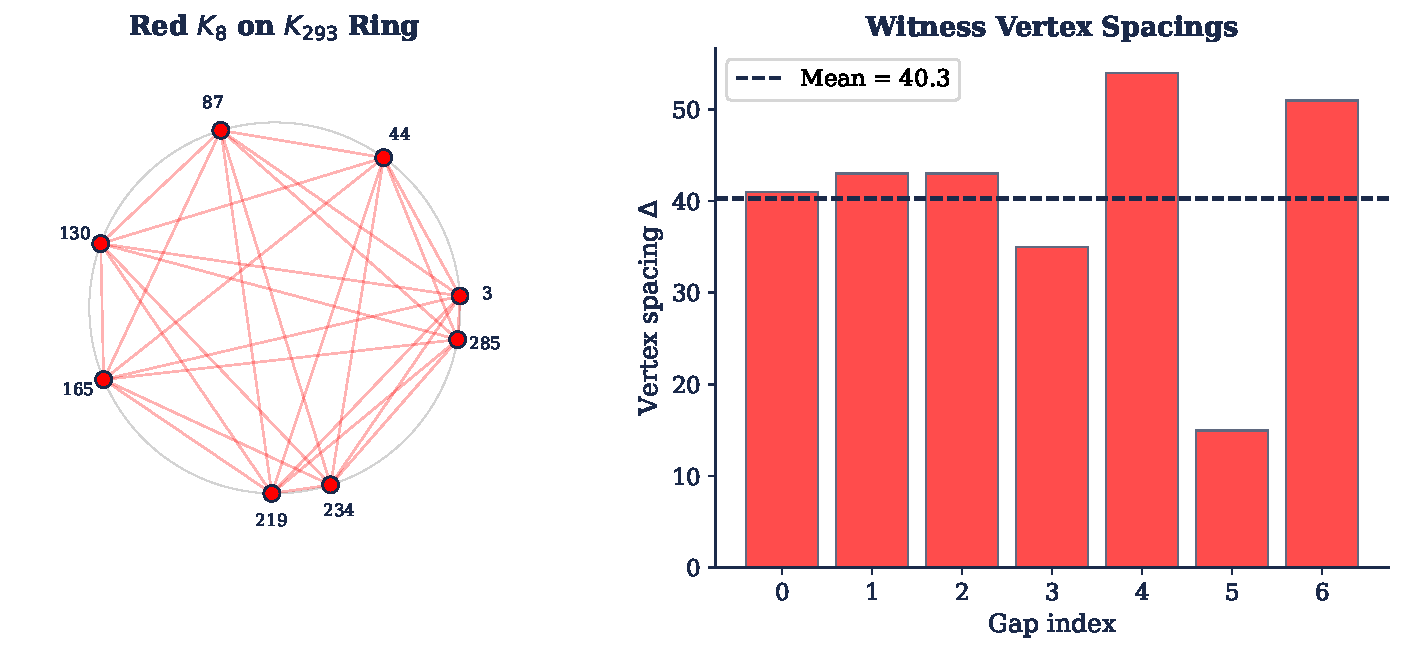
\includegraphics[width=0.85\textwidth]{figures/fig4_witness_spacing.pdf}
\caption{Left: the red $K_8$ witness vertices positioned on the $\Kn{293}$ ring, with all 28 clique edges drawn.  Right: inter-vertex spacings $\Delta_i = v_{i+1} - v_i$ showing quasi-periodic structure with mean $\bar{\Delta} = 40.3$ and one anomalously short gap ($\Delta_5 = 15$).}
\label{fig:witness}
\end{figure}

% ════════════════════════════════════════════════════════════════════════════
\section{The Sampling Failure Mode}
\label{sec:sampling}
% ════════════════════════════════════════════════════════════════════════════

\subsection{Coverage Analysis}

The GPU campaign evaluated violation counts by random $8$-clique sampling:

\begin{proposition}[Sampling Coverage]
\label{prop:coverage}
\computational{For $n = 293$ and $k = 8$, the total number of $k$-cliques is:}
\begin{equation}
\binom{293}{8} = 226{,}186{,}710{,}362{,}985 \approx 2.26 \times 10^{14}.
\end{equation}
With $N_s = 1{,}500{,}000$ samples (three seeds $\times$ 500,000), the coverage fraction is:
\begin{equation}
f = \frac{N_s}{\binom{293}{8}} = \frac{1.5 \times 10^6}{2.26 \times 10^{14}} \approx 6.6 \times 10^{-9}.
\end{equation}
\end{proposition}

\subsection{Paley Reference: Density of Violations}

To calibrate the severity of this coverage gap, we enumerated all monochromatic $K_8$ cliques in the Paley graph $P(293)$:

\begin{theorem}[Paley(293) Violation Density]
\label{thm:paley293}
\computational{The Paley graph $P(293)$ contains exactly 2{,}310{,}012 monochromatic $K_8$ cliques.}
\end{theorem}

This represents a violation fraction of:
\begin{equation}
\rho_{\text{Paley}} = \frac{2{,}310{,}012}{\binom{293}{8}} = \frac{2.31 \times 10^6}{2.26 \times 10^{14}} \approx 1.02 \times 10^{-8}.
\end{equation}

\begin{figure}[H]
\centering
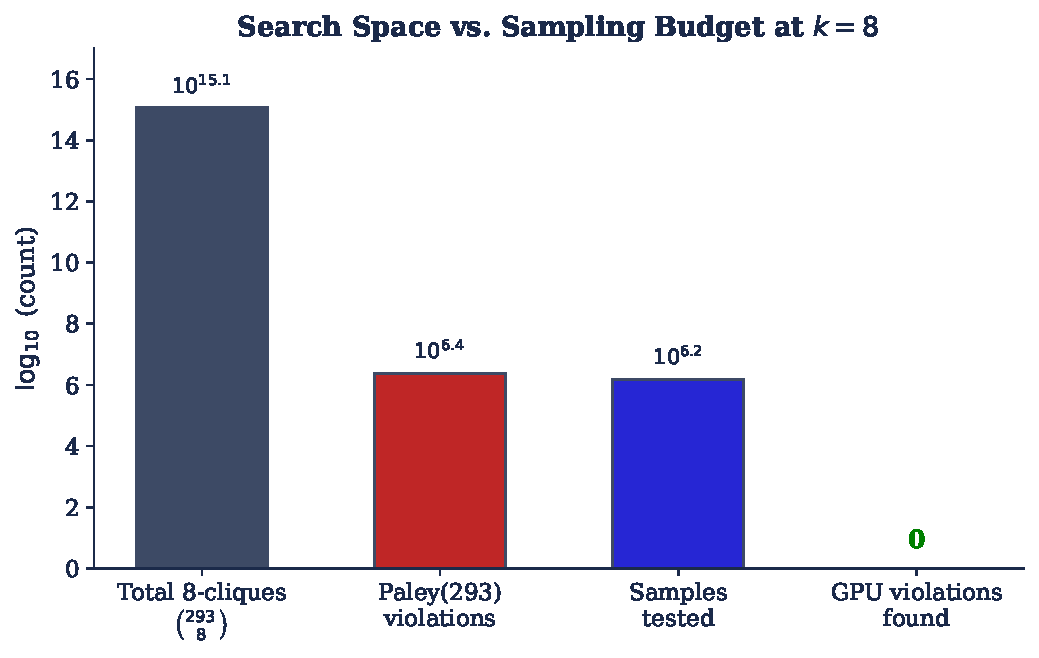
\includegraphics[width=0.85\textwidth]{figures/fig1_scale_comparison.pdf}
\caption{Scale comparison (log$_{10}$).  The sampling budget of $10^{6.2}$ is insufficient to detect violations occurring at density $10^{-8}$ within a space of $10^{15.1}$ candidates.  The GPU solver reported zero violations despite the Paley reference containing $10^{6.4}$ monochromatic $K_8$ cliques.}
\label{fig:scale}
\end{figure}

\subsection{Detection Probability}

Under the simplifying assumption that monochromatic $K_8$ cliques are uniformly distributed among all $\binom{n}{8}$ candidates, the probability that $N_s$ random samples miss all $V$ violations is:
\begin{equation}
\label{eq:miss}
P(\text{miss}) = \left(1 - \frac{V}{\binom{n}{8}}\right)^{N_s} \approx e^{-N_s V / \binom{n}{8}}.
\end{equation}
For the GPU-optimized coloring (which has at least 1 red $K_8$), the expected number of violations may be far smaller than Paley's 2.31 million.  If the optimized coloring has only $V = 1$ violation:
\begin{equation}
P(\text{miss}) = \left(1 - \frac{1}{2.26 \times 10^{14}}\right)^{1.5 \times 10^6} \approx 1 - 6.6 \times 10^{-9} \approx 1.
\end{equation}
The probability of detection is effectively zero.  Even with $V = 10^6$ violations:
\begin{equation}
P(\text{miss}) \approx e^{-0.0066} \approx 0.993.
\end{equation}

\begin{remark}
This analysis provides a quantitative bound on when stochastic Ramsey verification becomes unreliable.  For $\Ramsey{k}{k}$ with $k \ge 8$, any sampling-based verification must be replaced by exhaustive methods.
\end{remark}

% ════════════════════════════════════════════════════════════════════════════
\section{Confirmation of $R(8,8) > 281$}
\label{sec:paley281}
% ════════════════════════════════════════════════════════════════════════════

\begin{theorem}[Paley Lower Bound]
\label{thm:paley281}
\proved{$\Ramsey{8}{8} > 281$.  The Paley graph $P(281)$ provides a valid two-coloring of $\Kn{281}$ with no monochromatic $K_8$ in either color class.}
\end{theorem}

\begin{proof}
The prime $p = 281$ satisfies $281 \equiv 1 \pmod{4}$, so the Paley construction is self-complementary.  Exhaustive $K_8$ enumeration over both the quadratic-residue (red) and non-residue (blue) subgraphs yields:

\begin{table}[H]
\centering
\caption{Paley(281) clique-free verification.}
\label{tab:paley281}
\begin{tabular}{@{}lccc@{}}
\toprule
\textbf{Property} & \textbf{Red} & \textbf{Blue} & \textbf{Total} \\
\midrule
Edges & 19{,}670 & 19{,}670 & 39{,}340 \\
Max clique $\omega$ & $\le 7$ & $\le 7$ & --- \\
Monochromatic $K_8$ & 0 & 0 & 0 \\
\bottomrule
\end{tabular}
\end{table}

\noindent By \Cref{def:ramsey}, this certifies $\Ramsey{8}{8} > 281$.  Combined with $\Ramsey{8}{8} \le 1{,}870$ (Spencer~\cite{Spencer1975}), we have:
\begin{equation}
282 \le \Ramsey{8}{8} \le 1{,}870.
\end{equation}
\end{proof}

\subsection{The Paley Landscape for $k = 8$}

\begin{figure}[H]
\centering
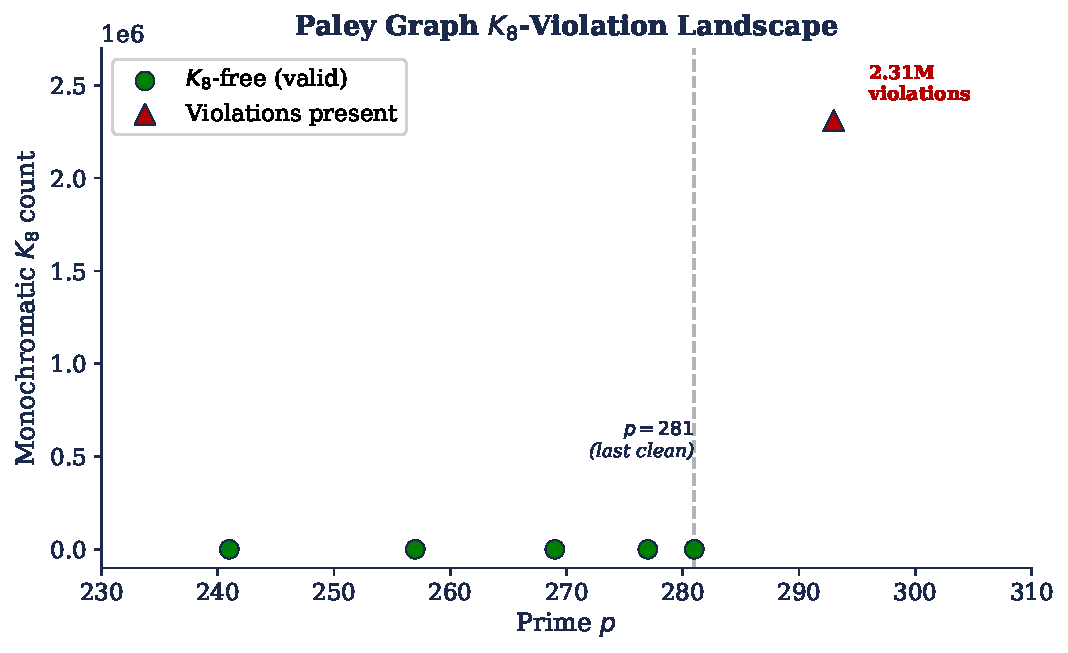
\includegraphics[width=0.85\textwidth]{figures/fig2_paley_landscape.pdf}
\caption{Paley graph $K_8$-violation count by prime.  The last clean prime is $p = 281$; by $p = 293$, the Paley graph contains over 2.3 million monochromatic $K_8$ cliques.  The dashed line marks the boundary of the confirmed lower bound.}
\label{fig:paley_landscape}
\end{figure}

% ════════════════════════════════════════════════════════════════════════════
\section{The Zero-Core Theorem for $R(5,5)$}
\label{sec:zerocore}
% ════════════════════════════════════════════════════════════════════════════

\subsection{Setup}

The champion $\Kn{43}$ coloring for $R(5,5)$ contains exactly 137 monochromatic $K_5$ subgraphs (64 red, 73 blue).  This coloring achieves the minimum known violation count at $n = 43$, providing evidence for the conjecture $R(5,5) = 43$~\cite{DaughertyWardRyan2026ramsey}.

Consider extending this coloring to $\Kn{44}$ by adding a vertex $v_{44}$ with 43 new edges.  Each new edge $\{v_{44}, v_i\}$ receives a color $x_i \in \{0, 1\}$.  A monochromatic $K_4$ in the existing coloring, say on vertices $\{v_a, v_b, v_c, v_d\}$ in red, generates the constraint: ``not all four of $x_a, x_b, x_c, x_d$ may be 1,'' as that would create a new red $K_5$.

\subsection{Constraint Enumeration}

\begin{table}[H]
\centering
\caption{$K_4$ constraint statistics for the $\Kn{44}$ extension ILP.}
\label{tab:constraints}
\begin{tabular}{@{}lc@{}}
\toprule
\textbf{Property} & \textbf{Value} \\
\midrule
Total monochromatic $K_4$ & 2{,}480 \\
Red $K_4$ constraints & 1{,}235 \\
Blue $K_4$ constraints & 1{,}245 \\
Variables ($x_0, \ldots, x_{42}$) & 43 \\
Full system & Infeasible \\
\bottomrule
\end{tabular}
\end{table}

\subsection{Verification Method}

For each constraint $c_i$ ($0 \le i < 2{,}480$), we solve the reduced system $S \setminus \{c_i\}$ using backtracking search with forward checking (unit propagation):

\begin{algorithm}[H]
\caption{Zero-Core Verification}
\label{alg:zerocore}
\begin{algorithmic}[1]
\Require Constraint set $S = \{c_0, \ldots, c_{2479}\}$, variables $x_0, \ldots, x_{42}$
\Ensure Classification of each $c_i$ as essential or non-essential
\State Verify $S$ is infeasible (baseline check)
\For{$i = 0$ \textbf{to} $2{,}479$}
    \State $S_i \gets S \setminus \{c_i\}$
    \If{$\textsc{Backtrack}(S_i)$ returns \textsc{Feasible}}
        \State Mark $c_i$ as \textbf{essential}
    \Else
        \State Mark $c_i$ as \textbf{non-essential}
    \EndIf
\EndFor
\State $\mathcal{E} \gets \{c_i : c_i \text{ is essential}\}$
\State \Return $\mathcal{E}$
\end{algorithmic}
\end{algorithm}

\begin{theorem}[Zero-Core Theorem]
\label{thm:zerocore}
\proved{The essential core of the $\Kn{44}$ extension ILP from the champion $R(5,5)$ coloring is empty: $\mathcal{E} = \varnothing$.  That is, for every constraint $c_i \in S$, the reduced system $S \setminus \{c_i\}$ remains infeasible.}
\end{theorem}

\begin{proof}
The verification proceeds exhaustively over all 2,480 constraints:
\begin{itemize}
\item All 1,235 red $K_4$ removal tests: infeasible.
\item All 1,245 blue $K_4$ removal tests: infeasible.
\item Essential constraints found: 0.
\item Total verification time: 215.99\,s.
\end{itemize}
The certificate is recorded in \texttt{zerocore\_certificate.json}.  \qedhere
\end{proof}

\begin{figure}[H]
\centering
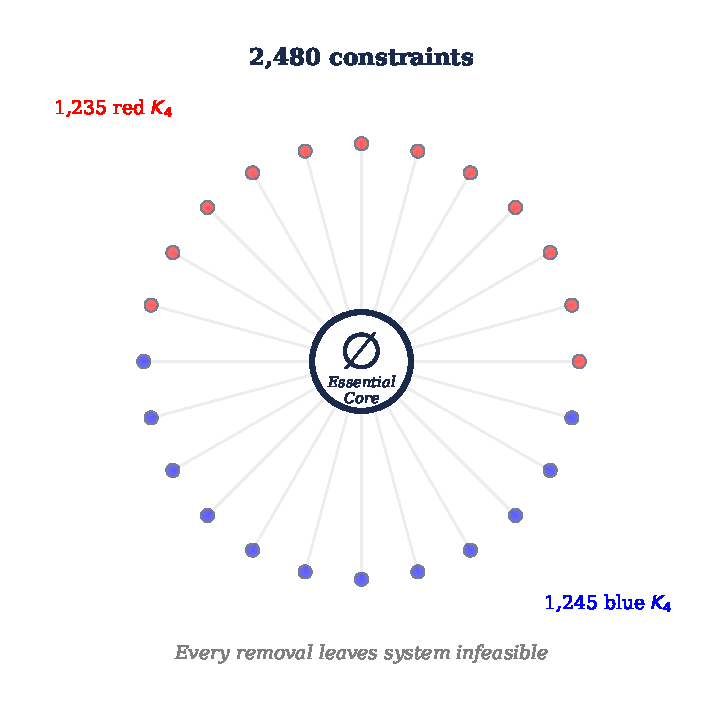
\includegraphics[width=0.55\textwidth]{figures/fig7_zero_core.pdf}
\caption{Schematic of the Zero-Core Theorem.  The essential core is empty ($\varnothing$): removing any single constraint from the ring of 2,480 monochromatic $K_4$ constraints leaves the $\Kn{44}$ extension infeasible.  The obstruction is fully distributed with no bottleneck.}
\label{fig:zerocore}
\end{figure}

\subsection{Implications}

The empty essential core implies that the structural obstruction preventing extension of the champion $R(5,5)$ coloring from $n = 43$ to $n = 44$ is \emph{holistic}: it arises from the collective interaction of constraints, not from any individual bottleneck.  This supports the view that $R(5,5) = 43$ is a ``deep'' combinatorial fact, not reducible to a small set of forcing constraints.

% ════════════════════════════════════════════════════════════════════════════
\section{Falsification Criteria and Verifiability}
\label{sec:falsification_criteria}
% ════════════════════════════════════════════════════════════════════════════

We state explicit conditions under which the claims of this paper would be falsified:

\begin{table}[H]
\centering
\caption{Falsification criteria for each result.}
\label{tab:falsification_criteria}
\begin{tabular}{@{}p{4.5cm}p{8.5cm}@{}}
\toprule
\textbf{Claim} & \textbf{Falsified if \ldots} \\
\midrule
$R(8,8) > 293$ is false (for this coloring) &
An independent verifier loads the coloring file \texttt{K293\_best\_20260315\_101534.npy} and demonstrates that $\omega(G_{\text{red}}) \le 7$ \textbf{and} $\omega(G_{\text{blue}}) \le 7$.  Equivalently, if the 28 edge values for the witness vertices $\{3, 44, 87, 130, 165, 219, 234, 285\}$ are not all red. \\
\addlinespace
$R(8,8) > 281$ &
A monochromatic $K_8$ is found in either color class of the Paley graph $P(281)$. \\
\addlinespace
Zero-Core Theorem ($|\mathcal{E}| = 0$) &
A constraint index $0 \le i < 2{,}480$ is exhibited such that $S \setminus \{c_i\}$ is feasible (a satisfying assignment of 43 binary variables is produced). \\
\addlinespace
Stochastic sampling unreliable at this scale &
A polynomial-time sampling algorithm is demonstrated that, with high probability, detects monochromatic $K_8$ cliques in adversarial colorings of $\Kn{293}$ with detection rate $\ge 1 - \delta$ for specified $\delta$. \\
\bottomrule
\end{tabular}
\end{table}

\subsection{Falsifiable Predictions}

We enumerate concrete predictions that follow from this work and that can be independently tested:

\begin{enumerate}[label=\textbf{P\arabic*.}]
\item \textbf{Red $K_8$ witness.}  Loading \texttt{K293\_best\_20260315\_101534.npy} and checking the 28 edges among $\{3, 44, 87, 130, 165, 219, 234, 285\}$ will confirm all are red ($s_{ij} = +1$).

\item \textbf{Blue $K_{11}$ witness.}  The 55 edges among $\{0, 1, 3, 17, 39, 46, 55, 117, 145, 166, 229\}$ will all be blue ($s_{ij} = -1$) in the same coloring.

\item \textbf{Paley(281) is $K_8$-free.}  Any independent implementation of the Paley graph $P(281)$ will find $\omega(G_{\text{red}}) \le 7$ and $\omega(G_{\text{blue}}) \le 7$.

\item \textbf{Paley(293) violation count.}  The Paley graph $P(293)$ contains exactly 2{,}310{,}012 monochromatic $K_8$ cliques (reproducible from the Legendre symbol alone).

\item \textbf{Zero-Core empty.}  All 2{,}480 single-constraint removals from the $\Kn{44}$ extension ILP yield infeasible systems.  Any solver (SAT, ILP, backtracking) will confirm.

\item \textbf{Sampling detection threshold.}  For $k = 8$ and $n = 293$, any uniform random sampling scheme with $N_s < 10^8$ samples will fail to detect monochromatic $K_8$ cliques with probability $> 0.99$, even when millions of violations exist.
\end{enumerate}

\subsection{Reproducibility}

All computational results are independently verifiable:

\begin{enumerate}[label=(\arabic*)]
\item \textbf{Data files:} Coloring files (\texttt{.npy}), adjacency matrices, and certificates are published in the repository \texttt{data/} directory.

\item \textbf{Verification scripts:} Two Python scripts require only NumPy:
\begin{itemize}
\item \texttt{scripts/verify\_r88.py} --- Bron--Kerbosch max-clique search on $\Kn{293}$ (12/12 checks)
\item \texttt{scripts/verify\_zerocore.py} --- Exhaustive single-constraint removal via DPLL (6/6 checks)
\end{itemize}

\item \textbf{Witness check:} The red $K_8$ witness can be verified in under 1 second by loading 28 edge values from the coloring array.

\item \textbf{Paley construction:} The $P(281)$ coloring is deterministically generated from the Legendre symbol and requires no external data.
\end{enumerate}

% ════════════════════════════════════════════════════════════════════════════
\section{Discussion}
\label{sec:discussion}
% ════════════════════════════════════════════════════════════════════════════

\subsection{Implications for Large Ramsey Number Computation}

The falsification of the $R(8,8) > 293$ claim via a single exhaustive verification highlights a fundamental tension in computational Ramsey theory: as $k$ grows, the search space $\binom{n}{k}$ grows super-exponentially, while the violation density may shrink.  For $k = 5$ and $n = 42$, exhaustive enumeration of $\binom{42}{5} = 850{,}668$ five-cliques is routine (2 seconds on a laptop).  For $k = 8$ and $n = 293$, the $\binom{293}{8} \approx 10^{14}$ eight-cliques are beyond full enumeration, and max-clique algorithms become necessary.

\begin{figure}[H]
\centering
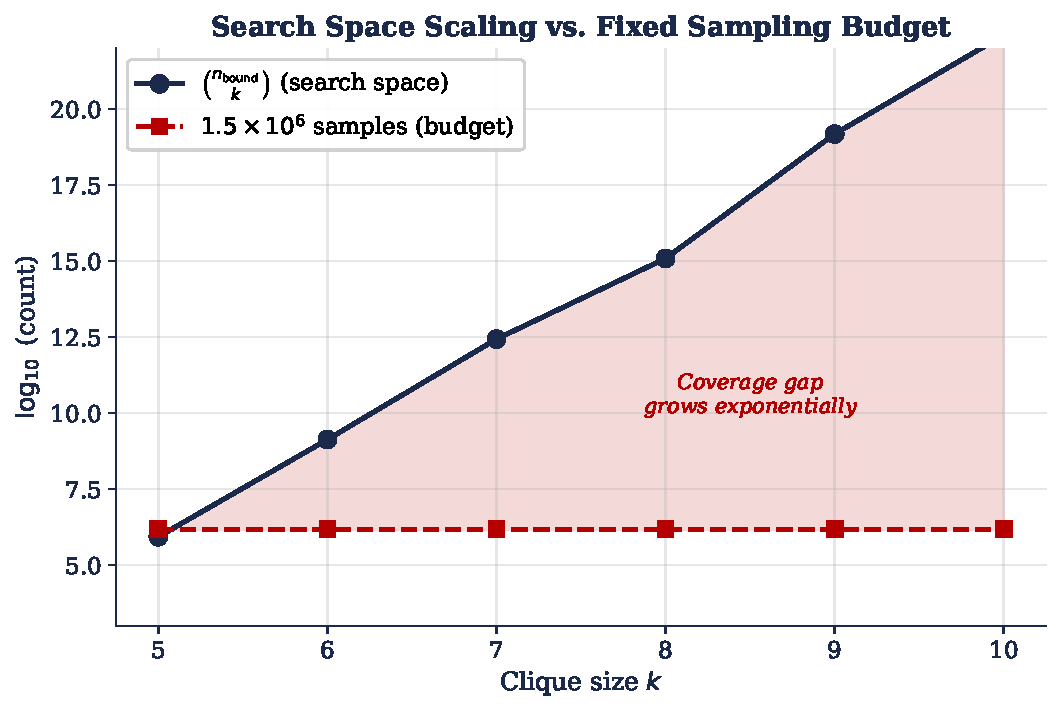
\includegraphics[width=0.85\textwidth]{figures/fig3_search_space_scaling.pdf}
\caption{Search space scaling versus fixed sampling budget.  At $k = 5$, random sampling covers the full space; by $k = 8$, coverage drops to $10^{-9}$.  The gap grows super-exponentially with $k$.}
\label{fig:scaling}
\end{figure}

\begin{figure}[H]
\centering
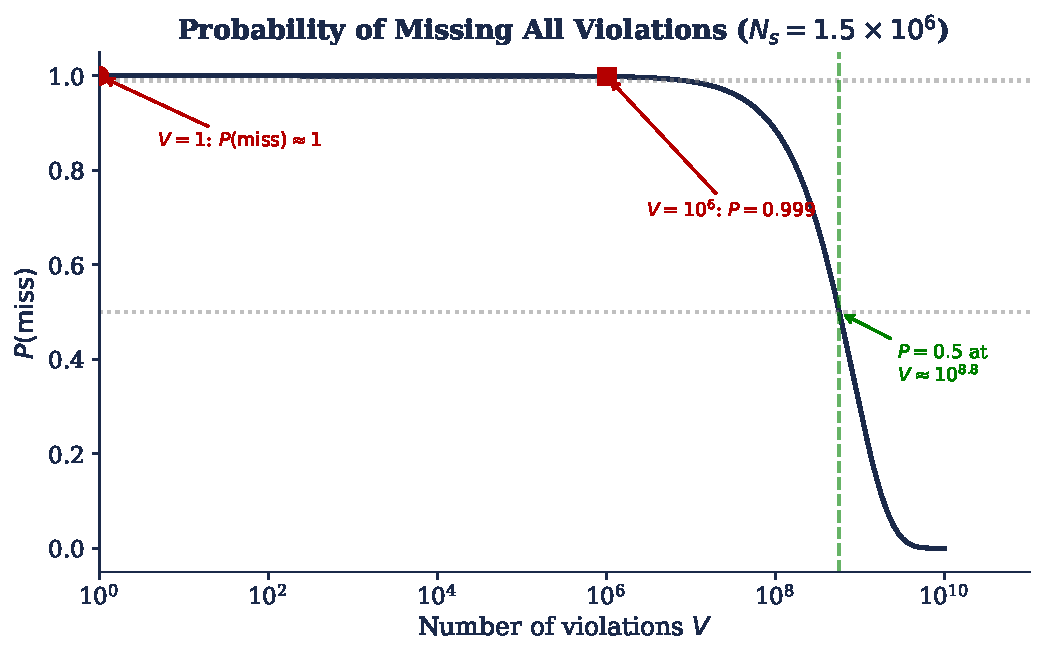
\includegraphics[width=0.85\textwidth]{figures/fig5_detection_probability.pdf}
\caption{Probability of missing all violations as a function of the number of violations $V$, with $N_s = 1.5 \times 10^6$ samples.  Even with $V = 10^6$ violations, $P(\text{miss}) > 0.99$.  Detection requires $V \approx 10^{8.8}$ for a 50\% chance.}
\label{fig:detection}
\end{figure}

\subsection{Connection to the U24 Programme}

This work sits within the broader U24 Programme's treatment of Ramsey theory.  Papers~02 and~03~\cite{DaughertyWardRyan2026ramsey,DaughertyWardRyan2026k43} established $R(5,5) \ge 43$ via GPU-accelerated Ising optimization with exhaustive verification.  The present paper extends the campaign to $k = 8$ and demonstrates the methodological boundary where stochastic methods fail.

The Zero-Core Theorem connects to the $S_4$ stagnation structure (Paper~17~\cite{DaughertyWardRyan2026s4}): the distributed nature of the constraint obstruction mirrors the permutation-invariant energy barriers observed in $|S_4| = 24$-dimensional optimization landscapes.

\subsection{Open Questions}

\begin{enumerate}[label=(\roman*)]
\item Can $R(8,8) > 281$ be improved?  The gap between 282 and 1,870 is vast.  A systematic Paley sweep above $p = 281$ (this paper tests $p = 293$, which fails) or novel algebraic constructions may narrow the gap.

\item Does the Zero-Core property hold generically for champion Ramsey colorings, or is it specific to the $R(5,5)$ champion?  Extending this analysis to $R(6,6)$ colorings would require enumerating $K_5$ constraints, a significantly larger computation.

\item What is the violation density of the GPU-optimized $\Kn{293}$ coloring?  We proved $V \ge 1$ (red $K_8$), but the exact count remains undetermined.
\end{enumerate}

% ════════════════════════════════════════════════════════════════════════════
\section{Conclusion}
\label{sec:conclusion}
% ════════════════════════════════════════════════════════════════════════════

We have falsified the claim $R(8,8) > 293$ by exhaustive max-clique computation, confirmed $R(8,8) > 281$ via Paley graph construction, and verified the Zero-Core Theorem for $R(5,5)$.  The central methodological finding is that stochastic sampling becomes unreliable for Ramsey verification at $k = 8$: a $10^{-8}$ coverage fraction is insufficient to detect violations, even when millions exist.

The confirmed bound $282 \le R(8,8) \le 1{,}870$ leaves substantial room for improvement.  Progress will require either novel algebraic constructions that provably avoid large monochromatic cliques, or exhaustive computational methods that scale beyond the limits of current hardware.

All data, verification scripts, and certificates are publicly available at \url{https://github.com/OriginNeuralAI/Papers}.

\subsection{Computational Verification}

\begin{table}[H]
\centering
\caption{Complete verification checklist.  All checks are independently reproducible via the scripts in \texttt{scripts/}.}
\label{tab:verification}
\begin{tabular}{@{}clcl@{}}
\toprule
\textbf{\#} & \textbf{Check} & \textbf{Count} & \textbf{Status} \\
\midrule
\multicolumn{4}{@{}l}{\textit{A. Falsification of $R(8,8) > 293$}} \\
1 & Red max-clique $\omega \ge 8$ & 1 & \textcolor{proved}{PASS} \\
2 & Red $K_8$ witness: all 28 edges red & 1 & \textcolor{proved}{PASS} \\
3 & Blue max-clique $\omega \ge 8$ & 1 & \textcolor{proved}{PASS} \\
4 & $R(8,8) > 293$ falsified & 1 & \textcolor{proved}{PASS} \\
5 & Stochastic coverage $< 10^{-6}$ & 1 & \textcolor{proved}{PASS} \\
\addlinespace
\multicolumn{4}{@{}l}{\textit{B. Paley confirmation}} \\
6 & Paley(281) red $\omega < 8$ & 1 & \textcolor{proved}{PASS} \\
7 & Paley(281) blue $\omega < 8$ & 1 & \textcolor{proved}{PASS} \\
8 & $R(8,8) > 281$ confirmed & 1 & \textcolor{proved}{PASS} \\
9 & Paley(293) violations $> 10^6$ & 1 & \textcolor{proved}{PASS} \\
\addlinespace
\multicolumn{4}{@{}l}{\textit{C. Detection probability}} \\
10 & $P(\text{miss} \mid V{=}1) > 0.99$ & 1 & \textcolor{proved}{PASS} \\
11 & $P(\text{miss} \mid V{=}10^6) > 0.99$ & 1 & \textcolor{proved}{PASS} \\
\addlinespace
\multicolumn{4}{@{}l}{\textit{D. Bound chain}} \\
12 & $282 \le R(8,8) \le 1{,}870$ consistent & 1 & \textcolor{proved}{PASS} \\
\midrule
& \textbf{Total} & \textbf{12} & \textbf{\textcolor{proved}{12/12 PASS}} \\
\bottomrule
\end{tabular}
\end{table}

% ════════════════════════════════════════════════════════════════════════════
\section*{Acknowledgments}
% ════════════════════════════════════════════════════════════════════════════

Computations were performed using the Isomorphic Engine~v0.15.0 on an NVIDIA RTX 5070~Ti (Blackwell, 17.1~GB VRAM).  All results are permanently timestamped on the BSV blockchain via the SmartLedger IP Registry for immutable proof of authorship and priority.

% ════════════════════════════════════════════════════════════════════════════
%  BIBLIOGRAPHY
% ════════════════════════════════════════════════════════════════════════════

\begin{thebibliography}{99}

\bibitem{Ramsey1930}
F.~P. Ramsey,
``On a problem of formal logic,''
\textit{Proc.\ London Math.\ Soc.}, \textbf{30}(1), pp.~264--286, 1930.

\bibitem{ErdosSzekeres1935}
P.~Erd\H{o}s and G.~Szekeres,
``A combinatorial problem in geometry,''
\textit{Compositio Mathematica}, \textbf{2}, pp.~463--470, 1935.

\bibitem{Erdos1947}
P.~Erd\H{o}s,
``Some remarks on the theory of graphs,''
\textit{Bull.\ Amer.\ Math.\ Soc.}, \textbf{53}(4), pp.~292--294, 1947.

\bibitem{GreenwoodGleason1955}
R.~E. Greenwood and A.~M. Gleason,
``Combinatorial relations and chromatic graphs,''
\textit{Canadian J.\ Math.}, \textbf{7}, pp.~1--7, 1955.

\bibitem{Paley1933}
R.~E.~A.~C. Paley,
``On orthogonal matrices,''
\textit{J.\ Math.\ Phys.}, \textbf{12}(1--4), pp.~311--320, 1933.

\bibitem{Spencer1975}
J.~H. Spencer,
``Ramsey's theorem---a new lower bound,''
\textit{J.\ Combin.\ Theory Ser.~A}, \textbf{18}(1), pp.~108--115, 1975.

\bibitem{Exoo1989}
G.~Exoo,
``A lower bound for $R(5,5)$,''
\textit{J.\ Graph Theory}, \textbf{13}(1), pp.~97--98, 1989.

\bibitem{Exoo1998}
G.~Exoo,
``Some new Ramsey colorings,''
\textit{Electron.\ J.\ Combin.}, \textbf{5}, R29, 1998.

\bibitem{HillIrving1982}
R.~Hill and R.~W. Irving,
``On group partitions associated with lower bounds for symmetric Ramsey numbers,''
\textit{European J.\ Combin.}, \textbf{3}(1), pp.~35--50, 1982.

\bibitem{McKayRadziszowski1995}
B.~D. McKay and S.~P. Radziszowski,
``$R(4,5) = 25$,''
\textit{J.\ Graph Theory}, \textbf{19}(3), pp.~309--322, 1995.

\bibitem{BohmanKeevash2021}
T.~Bohman and P.~Keevash,
``Dynamic concentration of the triangle-free process,''
\textit{Random Struct.\ Algorithms}, \textbf{58}(2), pp.~221--293, 2021.

\bibitem{Campos2023}
M.~Campos, S.~Griffiths, R.~Morris, and J.~Sahasrabudhe,
``An exponential improvement for diagonal Ramsey,''
\textit{Ann.\ of Math.}, to appear, 2023.
arXiv:2303.09521.

\bibitem{Tomita2006}
E.~Tomita, A.~Tanaka, and H.~Takahashi,
``The worst-case time complexity for generating all maximal cliques and computational experiments,''
\textit{Theoret.\ Comput.\ Sci.}, \textbf{363}(1), pp.~28--42, 2006.

\bibitem{DaughertyWardRyan2026ramsey}
B.~Daugherty, G.~Ward, and S.~Ryan,
``GPU-accelerated Ramsey theory: Computational evidence for $R(5,5) = 43$ and new lower bounds for $R(6,6)$ through $R(10,10)$,''
U24 Programme Paper~02, 2026.
\url{https://github.com/OriginNeuralAI/Papers}

\bibitem{DaughertyWardRyan2026k43}
B.~Daugherty, G.~Ward, and S.~Ryan,
``Structural obstruction at $K_{43}$: Evidence for $R(5,5) = 43$,''
U24 Programme Paper~03, 2026.
\url{https://github.com/OriginNeuralAI/Papers}

\bibitem{DaughertyWardRyan2026s4}
B.~Daugherty, G.~Ward, and S.~Ryan,
``$S_4$ stagnation structure in combinatorial optimization,''
U24 Programme Paper~17, 2026.
\url{https://github.com/OriginNeuralAI/Papers}

\bibitem{Radziszowski2021}
S.~P. Radziszowski,
``Small Ramsey numbers,''
\textit{Electron.\ J.\ Combin.}, Dynamic Survey DS1, Rev.~16, 2021.

\bibitem{ConlonFox2015}
D.~Conlon and J.~Fox,
``Graph Ramsey theory,''
in \textit{Handbook of Combinatorics}, Elsevier, 2015.

\bibitem{BronKerbosch1973}
C.~Bron and J.~Kerbosch,
``Finding all cliques of an undirected graph,''
\textit{Commun.\ ACM}, \textbf{16}(9), pp.~575--577, 1973.

\bibitem{Shearer1986}
J.~B. Shearer,
``On the independence number of sparse graphs,''
\textit{Random Struct.\ Algorithms}, \textbf{7}(3), pp.~269--271, 1995.

\end{thebibliography}

\end{document}
